\documentclass[tikz,convert={outfile=\jobname.svg}]{standalone}
\usepackage{mathtools}
\usepackage{amsfonts}
\usepackage{arydshln}

\usetikzlibrary{calc,positioning}
\begin{document}
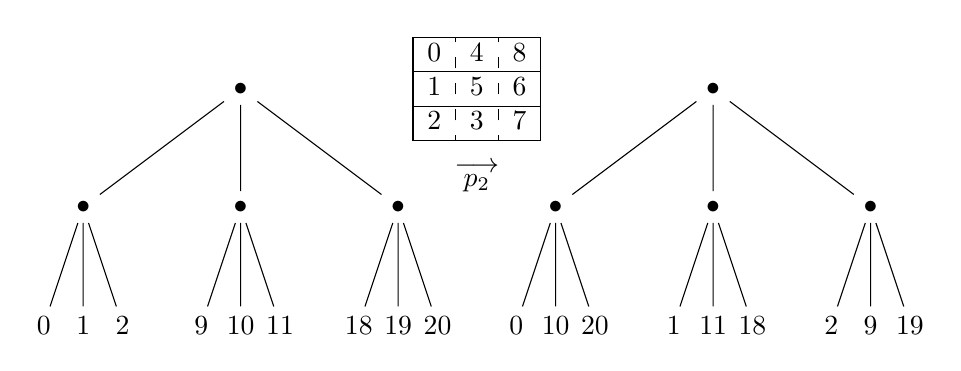
\begin{tikzpicture}
  \node (src) {$\bullet$}[sibling distance=20mm]
    child {node {$\bullet$}[sibling distance=5mm]
      child {node {0}}
      child {node {1}}
      child {node {2}}
    }
    child {node {$\bullet$}[sibling distance=5mm]
      child {node {9}}
      child {node {10}}
      child {node {11}}
    }
    child {node {$\bullet$}[sibling distance=5mm]
      child {node {18}}
      child {node {19}}
      child {node {20}}
    }
    ;

    \node[xshift=60mm] (trg) {$\bullet$}[sibling distance=20mm]
      child {node {$\bullet$}[sibling distance=5mm]
        child {node {0}}
        child {node {10}}
        child {node {20}}
      }
      child {node {$\bullet$}[sibling distance=5mm]
        child {node {1}}
        child {node {11}}
        child {node {18}}
      }
      child {node {$\bullet$}[sibling distance=5mm]
        child {node {2}}
        child {node {9}}
        child {node {19}}
      }
      ;

    \node[yshift=-10mm] (arr) at ($(src)!0.5!(trg)$) {$\longrightarrow$};
    \node[yshift=-2mm] at (arr) {$p_2$};
    \node[yshift=10mm] at (arr) {$\begin{array}{|c:c:c|}\hline 0 & 4 & 8 \\\hline 1 & 5 & 6 \\\hline 2 & 3 & 7 \\\hline\end{array}$};
\end{tikzpicture}

\end{document}
